\documentclass[11pt, a4paper,twocolumn]{jarticle}
\usepackage[dvipdfmx]{graphicx}
\usepackage{listings,jlisting}

\lstset{%
  language={C++},
  basicstyle={\small},%
  identifierstyle={\small},%
  commentstyle={\small\itshape},%
  keywordstyle={\small\bfseries},%
  ndkeywordstyle={\small},%
  stringstyle={\small\ttfamily},
  frame={tb},
  breaklines=true,
  columns=[l]{fullflexible},%
  numbers=left,%
  xrightmargin=0zw,%
  xleftmargin=3zw,%
  numberstyle={\scriptsize},%
  stepnumber=1,
  numbersep=1zw,%
  lineskip=-0.5ex%
}

\begin{document}
%=============================================================
\section{Learnig basic C programing ($1^{st} day$)}

\subsection{Purpose}
今回の実験ではC言語プログラミングの基本的な操作を理解する.

\subsection{Procedure}
まずWindows OS のノートパソコンを用意し"Visual C++ 2010 Express"を起動する.
その後与えられた1.1から1.3の課題に取り組む. \\
\textbf{Task 1.1} \\
整数1から12234までの総和を表示せよ. \\

\noindent
\textbf{Task 1.2} \\
1から100までの数を配列に格納したのち奇数の総和を表示せよ.

\noindent
\textbf{Task 1.3} \\
1000個の点をとることにより正弦波(振幅=1,位相=0)5波長分の値をtextファイルに出力しその出力結果をエクセルを用いて表示せよ.
\subsection{Result}
実験の結果まず,task 1.1では74841495の値が得られた.

またtask 1.2では25000の値が得られた.

さらにtask 1.3では図\ref{fig:1}のようなグラフがエクセルにより得られた.

\begin{figure}[htbp]
 \begin{center}
  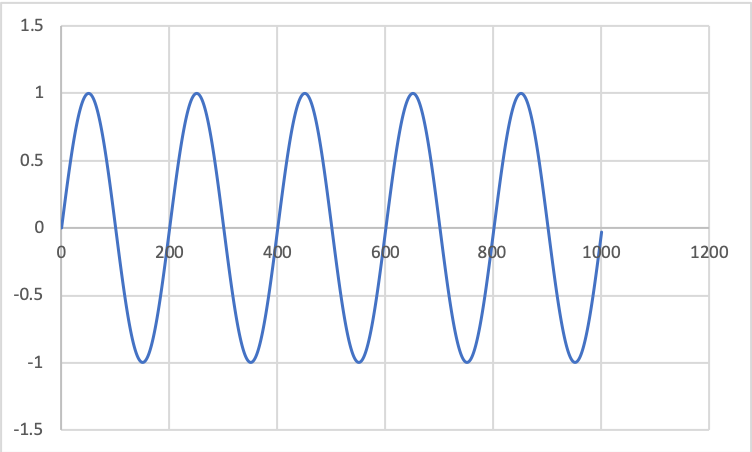
\includegraphics[width=0.8\linewidth]{fig1.png}
 \end{center}
 \caption{振幅=1,位相=0の正弦波}
 \label{fig:1}
\end{figure}

\subsection{Discussion}
今回の課題task1.1において1から12234までの総和をfor文を用いて計算を行なったが総和の公式から以下のようにも書き換えられることが予想できる.
\begin{eqnarray}
    \sum_{k=1}^{n} k = \frac{n(n+1)}{2} \nonumber
\end{eqnarray}
この数式を用いて総和を求める場合の計算時間はO(1)で計算できる一方でfor文を用いて総和を求める場合はO(N)の時間がかかることが予想できる.
またこの数式にn=12234を代入すると確かに74841495の値を得ることができるので今回の結果は正しいと考えられる.

また,task1.2においても前問同様に総和の公式を用いると
\begin{eqnarray}
    \sum_{k=1}^{n} 2k-1 & = & 2\frac{n(n+1)}{2} - n \nonumber \\
                        & = & n^2
\end{eqnarray}
この式においてn=50を代入すると2500の値が得られるのでプログラムによる計算結果は正しいと考えられる.
また,今回も同様に総和公式を使った場合の最悪時間計算量はO(N)で抑えられることができる.

\subsection{Appendix}
今回の課題で使用したソースコードを以下に示す.

\begin{lstlisting}[caption=task1.1,label=task1.1]
#include <iostream>
#include <math.h>
int main(){
    int sum = 0;
    for(int i=1; i<=12234;i++)
    {
        sum += i;
    }
    cout << sum << endl;
}
\end{lstlisting}

\begin{lstlisting}[caption=task1.2,label=task1.2]
#include <iostream>
#include <math.h>
int main(){
    int sum = 0, a[100];
    for(int i = 0; i < 100; i++){
        a[i] = i + 1;
        if(i%2 == 0){
            sum += a[i];
        }
    }
    cout << sum << endl;
}
\end{lstlisting}
\newpage
\begin{lstlisting}[caption=task1.3,label=task1.3]
#include <iostream>
#include <stdio.h>
#include <math.h>
#define PI 3.141592653
int main(){
    double a[1000];
    FILE *fp;
    fp = fopen("test.txt","w");
    for(int i = 0; i < 1000; i++)
    {
        a[i] = sin(PI*i/100);
    }
    for(int i = 0; i < 1000; i++)
    {
        fprintf(fp,"%f\n",a[i]);
    }
    fclose(fp);
}
\end{lstlisting}

%=============================================================
\newpage
\end{document}
